%!TEX root = project.tex

\chapter*{About this project}
\paragraph{Abstract}
A brief description of what the project is, in about two-hundred and fifty words.

\paragraph{Authors}
Explain here who the authors are.

\chapter{Background}
 \cite{galwayTourism} Galway City originally formed from a small fishing village located in the area near the Spanish Arch called ‘The Claddagh’ where the River Corrib meets Galway Bay. Galway later became a walled town in the year 1232 after the territory was captured by the Anglo Normans lead by Richard De Burgo. The town walls, some sections of which can be seen today near the Spanish Arch, were constructed circa 1270. A charter was granted in 1396 by Richard II which transferred governing powers to 14 merchant families, known locally as the 14 tribes of Galway. 
 The 14 tribes relished their independence but retained their close links to the British crown. Galway's strategic coastal location and natural harbour area resulted in a successful trade with both Portugal and Spain and the city prospered for centuries. However in 1651 with the arrival of Cromwell the region entered a long period of decline. Other prominent sea ports emerged on the east coast, namely Dublin and Waterford and trade with Spain came almost at an end. Many years would pass before Galway would again enjoy such prosperity but the legacy of the cities long and colourful history is evident in the character and style of the city. 
 Galway City is a thriving, bohemian, cultural city on the western coast of Ireland. Along with being a popular seaside destination with beautiful beaches and long winding promenade, it also has a buzzing cosmopolitan city centre. The city is a joy to explore with its labyrinthine cobbled streets, colourful shop facades and busy café/ bar culture.  The city is also well known for its many festivals throughout the year with huge crowds gathering for the annual Galway Arts Festival, Races and numerous other events. Old Ireland is present too with turf fires and traditional music featuring in many pubs to compliment your enjoyment of a well-earned pint of Guinness. Take an evening stroll along the promenade and watch the sunset over Galway Bay or watch the salmon fishermen in the River Corrib from the perfect vantage point of the Salmon Weir Bridge.
\cite{galway20} Galway is certainly one of the best tourist attraction in europe because of its rich cultures, traditions, festivals. Galway  and is bidding to become the European Capital of Culture in 2020.The bid represents an opportunity for everyone to join their hands together as a community and reflect and spread the uniqueness of our Galway culture and the richness, vitality and diversity of our shared European culture. \cite{failteireland}Failte Ireland has provided the regional tourism performance of 2014.  The overseas visitor to counties in 2014 shows that, there were total of 1235 people visiting Galway, and ranks 3rd in Ireland after Dublin (4,119) and Cork (1,542). Failte Ireland  has also provided the result of Overseas visitor revenue  (€mn) by county in 2014.  Adapted from : 
	INSERT IMAGE HERE


About Galway Civic Trust:  \cite{galway20}Dúchas na Gaillimhe - Galway Civic Trust is committed to protecting and enhancing Galway's natural, built and cultural heritage for the benefit of all. The Trust adopts a hands-on approach and undertakes improvement projects which otherwise would not happen. Our offices are located in the Latin Quarter at the Red Earl's Hall archaeological site.
Established in 1992, we have completed over 50 projects, ranging from the erection of historic wall plaques to the refurbishment of Rusheen Bay Bird Sanctuary and restoration of the Fishery Tower at Wolfe Tone Bridge.
In partnership with the Department of Social Protection, Galway City Council and Galway County Council, Galway Chamber of Commerce and Industry, The Heritage Council of Ireland, and the local community, we undertake works for the enhancement of Galway city and county.

\chapter{Introduction and Context}
	\section {General Problem Statement}
	\section {Previous work}
	\section {Purpose}
	\section {Scope}
	\section {Roadmap}

		
The introduction should be about three to five pages long.
Make sure you use references~\cite{einstein}

\chapter{Methodology}
About one to two pages.
Describe the way you went about your project:
\begin{itemize}
	\item Agile / incremental and iterative approach to development. Planning, meetings.
	\item What about validation and testing? Junit or some other framework.
	\item If team based, did you use GitHub during the development process.
	\item Selection criteria for algorithms, languages, platforms and technolo-gies.
\end{itemize}
Check out the nice graphs in Figure \ref{tikz:graphs}, and the nice diagram in Figure \ref{tikz:mydiagram}.

\begin{figure}
	\centering
	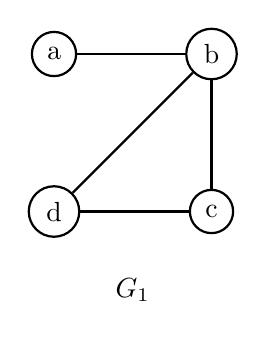
\begin{tikzpicture}
	\begin{scope}[every node/.style={circle,thick,draw}]
	\node (a) at (0,2) {a};
	\node (b) at (2,2) {b};
	\node (c) at (2,0) {c};
	\node (d) at (0,0) {d};
	\end{scope}
	\begin{scope}[every edge/.style={draw=black,thick}]
	\path (a) edge (b);
	\path (b) edge (c);
	\path (b) edge (d);
	\path (c) edge (d);
	\end{scope}
	\node () at (1,-1) {$G_1$};
	\end{tikzpicture}
	\hspace{1.5cm}
	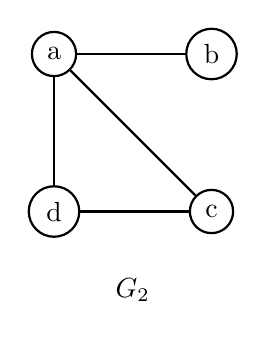
\begin{tikzpicture}
	\begin{scope}[every node/.style={circle,thick,draw}]
	\node (1) at (0,2) {a};
	\node (2) at (2,2) {b};
	\node (3) at (2,0) {c};
	\node (4) at (0,0) {d};
	\end{scope}
	\begin{scope}[every edge/.style={draw=black,thick}]
	\path (1) edge (2);
	\path (1) edge (3);
	\path (1) edge (4);
	\path (3) edge (4);
	\end{scope}
	\node () at (1,-1) {$G_2$};
	\end{tikzpicture}
	\caption{Nice pictures}
	\label{tikz:graphs}
\end{figure}


\begin{figure}
	\centering
	\begin{tikzpicture}[node distance=6cm]
	\node (a) [rect] {A Big Blue Block};
	\node (b) [oval, right of=a] {And His Oval Friend};
	\draw [line] (a) -- (b);
	\end{tikzpicture}
	\caption{Nice pictures}
	\label{tikz:graphs}
\end{figure}


\chapter{Technology Review}
	\section{Prototyping Tool - Justin-mind}
	\section{MEAN-Stack}
		\subsection{NoSql Technology - MongoDB}
		\subsection{Express.js}
		\subsection{Node.js}
		\subsection{AngularJs}
		\section{REST- Architecture}
		\section{JWT - JSON Web Tokens Authentication}
		\section{Send-grid - Email Delivery}
		\section{Cross-Platform Development}
		\section{Google Maps}
	
About seven to ten pages.
\begin{itemize}
	\item Describe each of the technologies you used at a conceptual level. Standards, Database Model (e.g. MongoDB, CouchDB), XMl, WSDL, JSON, JAXP.
	\item Use references (IEEE format, e.g. [1]), Books, Papers, URLs (timestamp) – sources should be authoritative. 
\end{itemize}


\chapter{System Design}
As many pages as needed.
	\section{Architecture}
		\subsection{Presentation Layer}
		\subsection{Business Logic }
		\subsection{Data Layer}
\begin{itemize}
	\item Architecture, UML etc. An overview of the different components of the system. Diagrams etc… Screen shots etc.
\end{itemize}

\begin{table}[h]
	\centering
	\begin{tabular}{x{2cm}p{3cm}}
		\toprule \\
		Column 1 & Column 2 \\
		\midrule \\
		Rows 2.1 & Row 2.2 \\
		\bottomrule
	\end{tabular}
	\caption{A table.}
	\label{table:mytable}
\end{table}

\chapter{System Evaluation}
As many pages as needed.
\begin{itemize}
	\item Prove that your software is robust. How? Testing etc. 
	\item Use performance benchmarks (space and time) if algorithmic.
	\item Measure the outcomes / outputs of your system / software against the objectives from the Introduction.
	\item Highlight any limitations or opportuni-ties in your approach or technologies used.
\end{itemize}

\chapter{Conclusion}
About three pages.

\begin{itemize}
	\item Briefly summarise your context and ob-jectives (a few lines).
	\item Highlight your findings from the evalua-tion section / chapter and any opportuni-ties identified.
\end{itemize}
